\chapter{Magnetically Driven Colloidal Systems}
\label{magneticallydrivencolloidalsystems}


We can see that biological active matter is effective at transporting or moving objects. The drawback, however, is that these systems always require a constant supply of energy. So far, there is no unlimited energy source available for this purpose. An exception are thermophoretic particles, which only need a beam of light to create a temperature gradient. In fact, some experiments have combined this principle with machine learning models, allowing particles to be guided toward a target region while reducing the impact of thermal noise~\cite{muinos2021reinforcement}. The limitation, though, is that only a relatively small number of particles can be manipulated in this way, which is not enough to drive something like a rotor.
Magnetism has long been a subject of interest because of its wide range of applications, from medical imaging and targeted drug delivery~\cite{geva2006magnetic, matthews2004functional, corti2011imaging} to lab-on-a-chip technologies~\cite{pamme2006magnetism}. More recently, it has also been used to control and organize colloidal systems. For example, Massana-Cid~\cite{massana2019tunable} showed that paramagnetic colloidal particles exposed to oscillating magnetic fields can self-assemble into large-scale “colloidal carpets”, as shown in Figure~\ref{fig:magneticallydrivencolloidalsystems}, that can move and even repair themselves. These carpets form because of the combined effects of magnetic dipole–dipole interactions and hydrodynamic coupling, and their degree of order can be tuned by changing the parameters of the external field.

This thesis focuses on paramagnetic colloids. Their key property is that the magnetic dipoles align with an external field, but once the field is removed, the dipoles lose their orientation and the material no longer shows magnetic order. The origin of this effect lies in the electronic and spin configuration of the atoms. A simple example is molecular oxygen, $O_2$, which has two unpaired valence electrons with the same spin. This imbalance leads to a net magnetic moment, giving rise to paramagnetism. The underlying principle is explained by Hund’s rule.

By themselves, paramagnetic particles cannot be considered active matter, even in the presence of a magnetic field. Several experiments have tried to induce motion in these systems, and one promising route is through Brownian rectification. For example, Tierno~\cite{tierno2012depinning} studied paramagnetic colloids placed above a ferrite garnet film, shown in Figure~\ref{fig:magneticallydrivencolloidalsystems}. The film contained permanent magnetic domains aligned along the $x$-axis, with alternating directions, while the colloids were subjected to a circularly precessing magnetic field in the $y$–$z$ plane.

With these parameters, and by varying only the driving frequency, four regimes of motion were identified. At the highest frequencies, the particles entered a pinned state, meaning the colloids did not translate. Tierno also tested elliptic magnetic fields and observed that, depending on the field magnitude, the particles displayed either attractive or repulsive interactions. These behaviors arise from the dipole–dipole potential between particles, given by

\begin{equation}
  U_{dd} = \frac{\mu}{4\pi} \left( \frac{\vec{m_i} \cdot \vec{m_j}}{x^3_{ij}} - \frac{3(\vec{m_i} \cdot \vec{x_{ij}})(\vec{m_j} \cdot \vec{x_{ij}})}{x^5_{ij}} \right),
\label{eq:dipolepairpotential}
\end{equation}

where $\vec{m_i}$ and $\vec{m_j}$ are the magnetic moments of particles $i$ and $j$, and $\vec{x_{ij}} = \vec{x_i} - \vec{x_j}$.

A subsequent study by Straube and Tierno~\cite{straube2013synchronous} provided a deeper understanding of these dynamics by analyzing the role of synchronization and thermal noise. Using the same ferrite garnet film with periodic magnetic domains, they investigated the motion of a single paramagnetic colloid driven by a rotating magnetic field. At low driving frequencies, the particle remained synchronized with the moving magnetic potential, resulting in constant-speed transport at the same velocity as the traveling landscape. Above a critical frequency, however, the particle lost synchronization, entering an asynchronous regime characterized by intermittent sliding and a reduced average speed.

\begin{figure}
  \begin{center}
    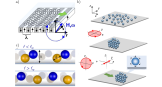
\includegraphics[width=0.95\textwidth]{figures/magneticallydrivencolloids.pdf}
  \end{center}
  \caption[Magnetically driven colloids examples.]{Panel a) shows the system with garnet films used to obtain net motion. The green arrow depicts the direction of the colloids, and the blue arrows show the magnetic field, obtained from~\cite{tierno2012depinning}. Panel b) show the process of how the colloids form a crystaline carpets and the direction of the film, depicted with the green arrow, due to the rotation of the rolling colloids, obtained from~\cite{massana2019tunable}. Panel c) shows spherical colloids in a confined space with different external field frequencies, obtained from~\cite{massana2020emergent}.}\label{fig:magneticallydrivencolloidalsystems}
\end{figure}


To describe these results, Straube and Tierno proposed a simplified analytical model based on the overdamped Langevin equation, which accounted for both deterministic forces and thermal fluctuations. Importantly, their model showed excellent agreement with experiments and revealed how thermal noise smooths the sharp transition between synchronous and asynchronous regimes. This highlights the interplay between deterministic driving and stochastic forces in rectification phenomena, and demonstrates how even passive colloids can be controlled and transported through external fields when symmetry is broken.

A year later, they used the same system with a rotating magnetic field whose ellipticity could be tuned~\cite{straube2014tunable}. The effect of this field was to create an asymmetric traveling potential that rectified Brownian motion and transported the particles across the surface.
One of the main results was that the interaction between particles could switch from repulsive to attractive just by adjusting the ellipticity of the field. In the attractive case, particles came together into stable doublets that moved with constant velocity along the magnetic stripes. They measured the dipolar forces that caused this binding and proposed a model that matched well with the experiments.
This shows that not only single-particle motion can be controlled, but also collective effects like chain formation and cooperative transport. The fact that this can be tuned with an external field suggests possible uses in microfluidics or lab-on-chip devices, where clustering or separation of particles can be useful for transport, mixing, or sorting.

More recently, Stoop~\cite{stoop2020collective} studied a dense monolayer of paramagnetic colloids driven above a triangular lattice of magnetic bubbles using a rotating magnetic field. The external field generated a two–dimensional traveling wave ratchet that transported the particles across the substrate. While single colloids showed no preferred direction of motion, collective interactions at higher densities led to a spontaneous symmetry breaking. In this regime, the particle current locked along one of the crystallographic axes of the lattice, producing a transversal current even though the driving direction was set between two symmetry axes.
They also reported that this locking could be polarized by adding a weak bias field, which made one direction energetically favorable over the other. At intermediate densities, elongated clusters of particles formed and moved coherently, showing that dipolar interactions stabilize directional locking. At very high densities, however, the effect was lost as the colloids formed a percolating network covering the entire substrate.
This work highlights how collective effects can generate robust directional transport that does not appear at the single-particle level. It shows that by controlling density and external fields, transport in colloidal systems can be tuned or polarized, which is useful for applications such as particle sorting and microfluidic control. 
%%%

An interesting study by Massana-Cid~\cite{massana2020emergent} analyzed the behavior of paramagnetic particles coated with nanoscale iron oxide grains confined within a space of suitable height, depicted in Figure~\ref{fig:magneticallydrivencolloidalsystems}, to prevent column formation while still allowing vertical (z-axis) motion. Under a static magnetic field, the particles tended to organize into triangular or square lattices~\cite{osterman2007observation}, and in some cases formed labyrinth-like structures. To avoid this ordering, the authors applied a conical time-dependent precessing magnetic field rotating around the z-axis. They found that the frequency of this field played a key role in the dynamics of the system: at certain frequencies, the particles exhibited collective rotation. However, because of the dense packing, strong interactions between neighboring particles significantly affected their motion.

The work of Ostinato~\cite{ostinato2024magnetically} can be seen as a continuation of the study by Massana-Cid, exploring the same type of confined paramagnetic colloids under precessing magnetic fields. While the first focused on the onset of collective rotation and structural organization, the latter extended the analysis to transport regimes and diffusion properties using equally both experiments and simulations.
Under a spatially isotropic field, the particles did not exhibit any net current but showed a strong increase in diffusion, up to sixty times higher than that of undriven colloids. This enhanced diffusion resulted from a continuous position exchange between particles near opposite walls, resembling a ``ceilidh dance''~\cite{meng2020field} of dimers that periodically bind and unbind.

%%%

In contrast, introducing a small spatial anisotropy by tilting the precession axis ($\delta \neq 0$) generated a robust bidirectional current. In this regime, colloids organized into two parallel flows moving in opposite directions, achieved by synchronized particle exchanges across the two planes. The magnitude of this current was highly tunable by varying both the driving frequency and the tilt angle, reaching maximal values when particles jumped exactly one lattice constant per field cycle. Remarkably, this bidirectional transport was robust against single-particle defects but could be disrupted by the introduction of ``magnetic holes'' (nonmagnetic inclusions in the ferrofluid), which acted as localized defects that broke the current pathways.

These results provide a powerful demonstration of how geometrical confinement and external field anisotropy can convert random thermal motion into ordered transport, without the need for field gradients. They highlight new opportunities for designing microfluidic devices where colloids could be directed, mixed, or sorted by simply tuning the parameters of an external homogeneous field.

%%%
